\documentclass{ltjsbook}
\usepackage{docmute} 
\usepackage{../../myStyle} 

\begin{document}
\chapter{Null hypothesis testing}
\label{m18_NHST}
Last time, I explained how to use a sample to estimate the population mean using an interval estimation method. This time, we will consider how to use it to determine whether there is a difference or not.

By estimating the mean value within a certain interval, it is possible to determine a range where it is predicted to be correct with a certain probability (XX%). If this estimation is performed for both the experimental and control groups, it can be said that the mean value of the experimental group is within this range, and that the mean value of the control group is within this other range.
Assuming there is no overlap in the ranges, we can confidently say that the average values of the experimental group and control group are different. However, it is natural for the confidence intervals to overlap. This raises the question of how to determine whether there is a significant difference or not.
This decision is called a "test" or "検定" in Japanese. Specifically, based on its format, it is referred to as the "Null Hypothesis Significance Test" or "帰無仮説検定" in Japanese, abbreviated as "NHST".

\label{ModelComparison1}
Where should we be careful? There are various issues, but let's illustrate one of them while explaining. Hypothesis testing is a type of \underline{model comparison}. A statistical model in this lecture is consistently explained as an idea of an ideal form plus errors for data, and a linear model, exemplified by regression analysis, is a representative model. Model comparison is the process of deciding which of the multiple models is better. Statistical testing, especially the \keytermE{null hypothesis significance test}, compares two models, a null hypothesis ($H_0$) and an alternative hypothesis ($H_1$), to determine which is better.

In other words, testing is an extension of estimation that incorporates judgement. Judgement is made based on some value or practical necessity.
For example, when developing new drugs as a measure against infectious diseases, it is necessary to make judgments such as "effective" or "ineffective" when determining whether or not they have an effect. This judgment is necessary because administering medication when there is no effect would be a waste of time and money, and could potentially have an impact on human life due to some kind of side effect.
Fortunately, in psychology, experiments that involve human life are almost impossible. However, they have been widely used to determine whether an experiment or intervention has an effect because they are easy to understand. While they are commonly used, their misuse and abuse have caused widespread problems. Due to the proliferation of misconceptions and poor practices, the American Statistical Association and the authoritative scientific journal Nature have issued statements declaring "Wrong usage is not allowed" \citep{wasserstein2016asa,amrhein2019scientists}, and some people even claim that "the statistics is dying" \citep{Toyoda202003}. It's important to note that null hypothesis testing isn't necessarily a flawed theory. The theory is logically valid, but it requires great care to implement and interprete correctly without violating theoretical assumptions. It should also be noted that the aforementioned statements focus on "p-value" and "statistical significance," not the significance test itself.

The fundamental cause of these misuses and abuses lies in the fact that null hypothesis significance testing provides a one-bit judgment of "effect is present" or "effect is not present". By assigning a Yes/No decision based on a particular criterion for estimation results that are ambiguous, the impact becomes too significant. For example, depending on the method, even a difference of 0.1 point in the mean difference between two groups may be judged as "there is a difference!". If this were a difference in height between two groups, 0.1 cm would be negligible, to the point of being effectively meaningless, but it might be conveyed as "there's a difference in growth between the group that received the intervention (medication) and the one that didn't!". Similarly, if this 0.1 point difference were in terms of average earnings (in units of 1 million yen) between men and women, the implications would be significantly different. In this case, there should not be any difference in earnings of even one yen between men and women. In other words, the question of whether there is a difference or not is actually a matter of domain knowledge, meaning it is dependent on the subject area being discussed, whether it is about biological height or industrial sociology wage systems, for example. And in cases where the field of study involves intangible subjects like psychology, it is challenging to come up with a unified resolution on how much quantity needs to be detected for it to be meaningful, and how much can be ignored. In psychology, it is crucial to emphasize that the estimation before making any judgments is essential and to ensure that one does not become distracted by flashy results that are reduced to a one-bit decision.


Well, I apologize for starting with a warning phrase. With that said, let's begin explaining things in more detail while keeping in mind what I previously wrote above.

% ここにあるように，2つのモデルを比較することになるのですが，ステップの最後の段階に「間違っているか正しいかを判断する」とあります。どのモデルがどれぐらい良いか，という程度の問題ではなく，「いいか，悪いか」「イエスか，ノーか」という1bit判断\footnote{1bitは第\ref{sec::4c}で説明したように，2進数のデジタルデータの最小単位で，0/1の2つの状態しかありません。}になってしまうこと，これがマズいのです。先ほども述べたように，差があるかどうかで言えば男女差はいろいろなところで検出\textbf{できます}。が，この場合どれほどあるのか，という大きさの方が問題なのです。やり方によっては，二群の平均身長の差が0.1cmでも「差がある！」と喚き立てることができます。普通はその程度の差は気にならないと思いますが，差が「ある」か「ない」かと言われれば，「ある」わけです。では僅かな差を気にしないようにすれば良いですか？ いいえ，そうでもなくて，たとえば平均獲得賃金であれば，男女差は1円だってあるべきではないのです。つまり，程度問題としてはドメイン知識\footnote{ドメインとはその領域のことです。生物学的な身長の話をしているのか，産業社会学的な賃金体系の話をしているのか，といった話題にまつわる領域のことだと思ってください}に照らし合わせて考えなければなりません。心理学のような目に見えない対象を研究する場合は，この判断が非常に難しく，どの程度の量であれば検出することに意味があるのか，どの程度なら無視して良いのか，ということについて，統一的な見解が作りにくい，という背景もあります。だからと言って，「ある」か「ない」か，だけの話にするのは危険だ，ということは肝に銘じておいてください。


% 前回は，帰無仮説と対立仮説という2つのモデルを戦わせる意思決定法，帰無仮説検定のやり方について導入的なお話をしました。今回は，これをいくつかの具体例に当てはめて考えていくことにしましょう。具体的な計算式や確率的な数字は，統計パッケージで自動的に計算されます。その利便性のおかげで，帰無仮説検定がさまざまな学問領域に広く行き渡ったことは既に指摘した通りですが，同時に「手続きが簡単だから，内容も簡単」だと思っていると，誤用・悪用になりますので，よく注意してください。例えるなら，車の運転がマニュアルトランスミッションからオートマチックになったことで，比較的簡単に運転できるようになりましたが，それで交通量が増えて事故が多発するようでは，かえって社会的には良くないことかもしれない，ということです\footnote{電子レンジの普及のように，簡単になって利便性が増し，危険性もそうない技術的なものもあります。車の例えも，危険性と利便性のバランスでいくと，十分許容範囲なのかもしれませんが，帰無仮説検定は利便性も危険性もどちらも大きい，ハイリスク・ハイリターンな技術なのです。}


% \section{帰無仮説検定Null Hypothesis Significance Test:NHST}

% 先回りしていうのも気が引けますが，この検定というのは古くから使われてきた方法で，さまざまな業界に広まった方法です。その理由は，計算プロセスが比較的単純であることから，多くの統計パッケージの中に組み込まれたからです。ただし，実践に際しては緻密な設計が必要であり，判断する上での多くの注意点が存在します。そういう意味で非常に繊細な技術なのですが，一方でボタンをポチポチと押すだけで瞬時に答えが出るものですから，とてもよく使われているのですが，\underline{多くの誤用・悪用}を生んでしまいました。あまりにも間違った使われ方，悪い使われ方が広まっていることから，アメリカ統計学会や権威ある科学雑誌であるNatureが「間違えた使い方はダメだぞ」という声明を出しており\citep{wasserstein2016asa,amrhein2019scientists}，「統計学は瀕死だ」という人もいるほどです\citep{Toyoda202003}。これから帰無仮説検定について学んでいきますが，みなさんはこれらの先人の過ちを繰り返さないように，慎重に慎重に読み進めていってください。念のためにいっておきますが，帰無仮説検定は間違った理論だ，というわけではありません。正しいのですが，理論的仮定を犯さずに実践し，正しく解釈するのに細心の注意が必要だ，ということです\footnote{これらの声明のタイトルもよく見ると，``p-valuie''($p$値)や``statistical significance''(統計的有意)について注意が必要だ，ということであって，帰無仮説検定``significance test''そのものが間違っているというわけではないのです。}\footnote{そんな危うい技術いやだよ，もう少し簡単なものないの，と言われると，幸いにして答えはYesです。その方法についても後ほど(第\ref{chapter25}講以降)説明しますが，最近できた代替方法に比べて帰無仮説検定の考え方の方が先に広まってしまっているため，これまでの心理学形の論文や今まさに掲載されている論文なども，帰無仮説検定を使って書かれているのがほとんどです。みなさんは先行研究を読むためにも，この技術を知らなければなりません。ただしこれらの先行研究は，過去(あるいは今も現在進行形で? )の「間違ったやり方」で結論が出ている可能性もある，と眉に唾しながら読み解く必要があるでしょう。}。


\section{Procedures for Hypothesis Testing}
The procedure of statistical null hypothesis testing generally proceeds with the following steps.
\begin{enumerate}
	\item 仮説を設定する。
	\item 統計的仮説検定に用いられる検定統計量を選択する。
	\item 仮説選定判断の基準になる確率を設定する。
	\item 実際のデータから検定統計量の実現値を計算する。
	\item 最初に定めた仮説を支持するかどうかを判断する。
\end{enumerate}


Let's look at each step in order.
\subsection{Setting hypotheses}
The first step is to set a hypothesis. In hypothesis testing, two hypotheses are prepared, the \keytermE{null hypothesis} and the \keytermE{alternative hypothesis}. Since the purpose of the test is to determine whether there is a difference or not, we compare the model that assumes there is a difference and the model that assumes there is no difference, and see which one comes out on top.

The null hypothesis is a hypothesis that is empty and void, as the word "null" suggests. It is a hypothesis that suggests there are no differences or effects when comparing typically. Against this, a null hypothesis is prepared, which suggests there are no differences or effects. The term "null hypothesis" was coined because it is a hypothesis that people would like to see disappear and become null and void.

In contrast, the alternative hypothesis is the possibility of another option or something different, and it becomes a hypothesis stating that "there is a difference" or "there is an effect". As a researcher, you would want to support this side. However, setting a null hypothesis such as NHST is a method of judgement in an indirect logical way. In other words, when thinking about setting a null hypothesis stating that there is no difference, if something strange occurs, the null hypothesis can be rejected and thus the alternative hypothesis can be adopted. This is the fundamental logic.

% 注意が必要なのは，もしかすると「効果がない」という研究がしたいことがあるかもしれない，ということですね。呪いやインチキはなかったんだ，ということを証明するのも科学の役割のような気がしますが，それではこの場合，なくなって欲しい帰無仮説は「差がある」で，対立仮説は「差がない」になるのでしょうか？ いいえ，そうはなりません。

% たとえば，二群の母平均に差があるかどうかを検定したいとしましょう。母平均をそれぞれ$\mu_1,\mu_2$とします。このとき，帰無仮説は$H_0 : \mu_1 = \mu_2$であり，対立仮説は$H_1:\mu_1 \neq \mu_2$になります。これをよく見てください。，帰無仮説と対立仮説は実は同等の仮説で戦っているわけではないことに気づきましたでしょうか。帰無仮説は「2つの母平均は一致する」と言ってます。対立仮説は「2つの母平均は一致しない」と言ってます。帰無仮説の「一致する」という言い方は，イコールの状態ですから，1つしかありません。これに対して対立仮説は「一致しない」としか言ってません。$\mu_1>\mu_2$なのか，$\mu_1<\mu_2$なのか，はたまた$\mu_1 > \mu_2 + 0.5$($\mu_1$と$\mu_2$は0.5以上離れている)なのか，あるいはもっと大きな，小さな差があるのかどうか・・・こうした詳細については何も言及していません。つまり，2つのモデル比較といいながら，実はフェアではなく，一方は$H_0 : \mu_1 = \mu_2$というモデル，他方はそれ以外全部，という非対称な関係があります。

% どうしてそうなるのか，というのはこの後の検定の実際のロジックを進めていく時の，計算方法の中で明らかになっていきますが，ともかく帰無仮説はこうした「2つの平均の差がない」という特殊な一点張りの状況に立脚するものですから，「差がない」という仮説は立てようがないのです。「差がない」，というのは差が0.1なのか0.2なのか0.3なのか0.31なのか0.32なのか，0.321なのか0.322なのか・・・というどの状況なのかが特定できないからです\footnote{面倒ですが，「差が0.3ジャストである」という帰無仮説vs「差が0.3ジャストではない」という対立仮説の勝負なら，帰無仮説検定の文脈で検証することはできます。計算が面倒で一般化できなくなりますし，差が0.31でも0.301でも0.3001でも違う計算をすることになりますので，実際的ではありませんが。}

% ともかくまずは，帰無仮説と対立仮説という2つを立てて戦わせる，というところを理解していただければと思います。

\subsection{Selecting a Test Statistic Used in Statistical Hypothesis Testing}
For example, depending on the research scenario, the sample statistics you want to consider may vary, such as whether you want to indicate a difference in mean, a difference in ratio, whether the correlation coefficient has meaning, or whether there is a difference in frequency distribution, etc.

If sample statistics cannot be compared directly, we must calculate a test statistic for hypothesis testing from those statistics. In previous examples, we used the t-distribution to estimate the mean for instance. When comparing means, the test statistic to be used is the t-value, which follows this t-distribution.
However, with some estimations, correlation coefficients may utilize distributions that are not simple. In such cases, even without considering parameter estimation or confidence intervals, it is possible to take a detour and convert to easily calculable statistical data to make decisions for hypothesis testing.

To test for correlation, we take this detour route and conduct a test using the $t$-distribution. We may also calculate other statistical values such as $F$ or $\chi^2$ (called chi-squared).

We rely on mathematical statistics to understand which statistical measures are needed in which scenarios, so the only way to learn is through memorization. However, on the flip side, if you know some typical examples, you can obtain results without requiring mathematical proofs. So, please take heart and energetically persevere in your studies.

\subsection{Establishing the probability that will serve as the criteria for selecting hypotheses}
\label{ModelComparison2}
Hypothesis testing is a competition that determines the superiority or inferiority based on model comparison. In considering the results of estimation, it is also a "practical decision-making tool" to decide which of the null hypothesis or alternative hypothesis to favor. Therefore, it is necessary to establish rules beforehand such as "let's consider it settled if it becomes like this." If the judgment rule is not decided beforehand, it will be troublesome if the rule changes later, so it is necessary to decide it beforehand.

This probability is called the \keytermE{significance level}. "Significant" means that it has statistical significance, indicating that there is a significant difference. The standard is to judge that the match is over if a greater difference is found. This is expressed in terms of probability, but in psychology, 5\% is generally used. Why 5? There is no particular reason. 6 or 4 could have been used instead, but the person who initially conducted the statistical test said "there is no basis, but let's start with 5 for now," and it is still being used. Therefore, there is no need to be particular about it, but sometimes numbers such as 1\%, 0.1\%, 10\% are used, although any number does not have a deep reason.

Just to clarify, these numbers are only criteria for judging superiority or inferiority, and are not numbers referring to the data itself. It's important to note that they are not a measure of the correctness of the hypothesis or the fitness of the hypothesis model with the data.

\subsection{Calculating the observed value of the test statistic from actual data}

We calculate the test statistic by plugging in actual data.
\subsection{Determining whether the initial hypothesis is incorrect or correct}
Until this point, we have been setting the rules. From here on, we will pit two models (hypotheses) against each other according to these rules.

Using actual data, we calculate the test statistic and the probability that it occurs, without modifying the TeX code. This probability is called the \keytermE{$p$-value}. The result of the hypothesis test depends on whether the $p$-value is above or below the significance level. By convention, we \keytermE{accept} the hypothesis of the winning side and \keytermE{reject} the other.

This is a series of steps. The procedure is formally established, so the statistical software automatically performs intermediate calculations. Thus, there is little effort required for calculations, but this also means that caution is necessary to avoid using it arbitrarily for results without careful consideration.

% 計算方法など，具体的な内容は次回になります。基本的な流れをまずは掴んでおいてください。このモデル比較は程度問題ではなく優劣の話であること，厳密に言えば統計的な話というより，実践上・実用上の意思決定の問題になっていることに注意が必要です。
% 既に述べたように，帰無仮説検定は，現代ではさまざまな角度から批判がなされています。その批判の1つが，モデルの当てはまりのよさや程度の話ではなくて，結局のところ採択か棄却か，という「勝ち負け」という紋切り型の二値判断になってしまうことです。論文などを読んでいて「統計的に差がある」と書いてあれば，なるほど差があるのでしょう，効果があるのでしょうと思って，その実際的な大きさまで考察しなくなることがあります。もしかすると，あなたの読む先行研究でもごく僅かな差を「差があったのだ！」と針小棒大に歌い上げているかもしれません。皆さんは，同じような過ちを犯さないように注意しつつ，作法としての帰無仮説検定をこれからしっかり身につけていってください。


\section{One-sample t-test}
Let's consider a specific example. First, we will look at testing using the standard normal distribution when the population's standard deviation is known, just like when estimating the mean. Then, we will look at testing using the t-distribution when we don't know the population's standard deviation.
\subsection{When the mother SD is known}
% ではまず，1つの平均値の推定を使って，検定をしてみましょう。「推定を使って検定」というのは変な表現に聞こえるかもしれませんが，推定は「母数はこれぐらいではないか」という予測の話であり，検定は「母数がそのようであれば，このように結論づける」という意思決定の話なのです\footnote{意思決定なんかしなくていいじゃない，と思うかもしれません。確かに科学的探究であれば，母数がどの程度であるかというのを知ることで十分なのです。しかし，帰無仮説検定は農学で生まれ，医学領域にも広まっている技術です。これ以上実験を続けて良いかどうか，この治療薬を投与し続けて良いかどうか，といった実際的な問題がそこにはあり，効果があるとしたらこれぐらい，ない可能性もなくはない...という態度を続けていると前に進まないので，何らかの基準が必要だという事情もあります。心理学においても，より実際的な場面では意思決定が必要になることもありましょう。}。

Now, let's give a specific example to move the discussion forward. Let's say a school conducted a literacy test and randomly selected 49 records, with an average score of 52. It's known that the national average for this test is 50 with an SD of 9, assuming a normal distribution. Comparing the school's performance directly with this information would suggest that the school is performing well, but the question here is whether we can draw such conclusions based on a difference of just two points.

Let's recall the steps of hypothesis testing. First, we set a hypothesis.
"What we want to do here is to determine whether this school's grades are good or not. In other words, since we know the distribution of the national average as the population and its average and SD, we want to know whether the sample means are the same as the population mean or different. Since it is a sample, there may be cases where high scores (and vice versa) are coincidental. Nonetheless, we want to know whether the difference between the inferred population mean from this sample mean and the theoretical average value of this test (national average) is statistically significant or not. Expressed in a formula, the sample mean is represented by $\bar{X}$, and is distributed as $\bar{X} \sim N(\mu, \frac{\sigma}{\sqrt{n}})$. Therefore, the null hypothesis is that $\mu=50$, and the alternative hypothesis is that $\mu \neq 50$."

The next item is the test statistic. In this case, we are estimating the mean value and comparing it to a normal distribution with a theoretical mean of 50 and a standard deviation of 9. Therefore, this is a special case where the characteristics of the target to be estimated are already known. If we transform this, it will follow a standard normal distribution, and the standardized Z-score will become the test statistic.

The third step was setting the reference probability. This is the decision of the rule that determines the winner and the loser. This is usually set to 0.05 (5%) without any particular meaning, following convention.

The preparation is now complete. It's time to calculate the actual test statistics. When the sample is drawn from a normally distributed population with mean $\mu$ and variance $\sigma^2$, the sample mean follows a normal distribution as well.
\[ \bar{X} \sim N(\mu,\frac{\sigma}{\sqrt{n}}) \]
You are a translator.
\[ 52 \sim N(50,9/\sqrt{49}) \]
It is believed that by standardizing, we can use the standard normal distribution.
\[ (52-50)/(9/7) \sim N(0,1) \]
We get $(52-50)/(9/7) = 2/1.285714 = 1.555...$. Rounding to three decimal places, we have 1.556. Where does this number lie?

Let's calculate the probability here. This is the next step, which is to calculate the observed value of the test statistic from actual data. In a standard normal distribution, the probability of getting a number greater than 1.556 is\footnote{This is a tricky area of probability, particularly with continuous variables. The probability of the number 1.556 appearing is actually zero, similar to the idea in Euclidean geometry that a point has position but not size. Probability is represented by area, so a more accurate description is the probability of getting a number \underline{greater than} 1.556.} $p=0.05985405$. In other words, the probability of getting a number greater than 1.556 in a standard normal distribution is 5.9%\footnote{This is calculated in R using the following formula: \texttt{1-pnorm(1.556,mean=0,sd=1)}}.

Finally, it's time for the verdict. The 5% was the threshold for determining statistical significance, but the "realized value of the random variable" obtained this time has a greater probability than 5%. In other words, it is a common story that a bigger value means a higher chance of appearing. It's not such a rare number. In other words, it is highly possible that this sample happens to be two points higher than the average. Although we might want to say that the students in this school are excellent, we cannot say with certainty that it is the case since such a difference might occur accidentally. Therefore, the null hypothesis wins, meaning that "the performance of this school is not particularly good" and "there is no statistical difference."

Let's confirm with a figure. Figure \ref{fig::18_01b} shows the standard normal distribution and the value associated with the judgment we made this time. The calculated statistic is standardized to the standard normal distribution. Considering the criterion of 5\% in the standard normal distribution, it becomes the area that exceeds $\pm1.96$. If the data for this time enters this area, the null hypothesis is rejected, but as the data did not enter this area, it cannot be rejected. The area where the null hypothesis is rejected is generally called the \textit{rejection region}, and the critical value, which is the borderline number that passes this area, is called the \textit{critical value}. The critical value for this time is $\pm1.96$, and since the value of 1.55 did not enter the rejection region, the null hypothesis wins.
\begin{figure}[ht]
	\centering
	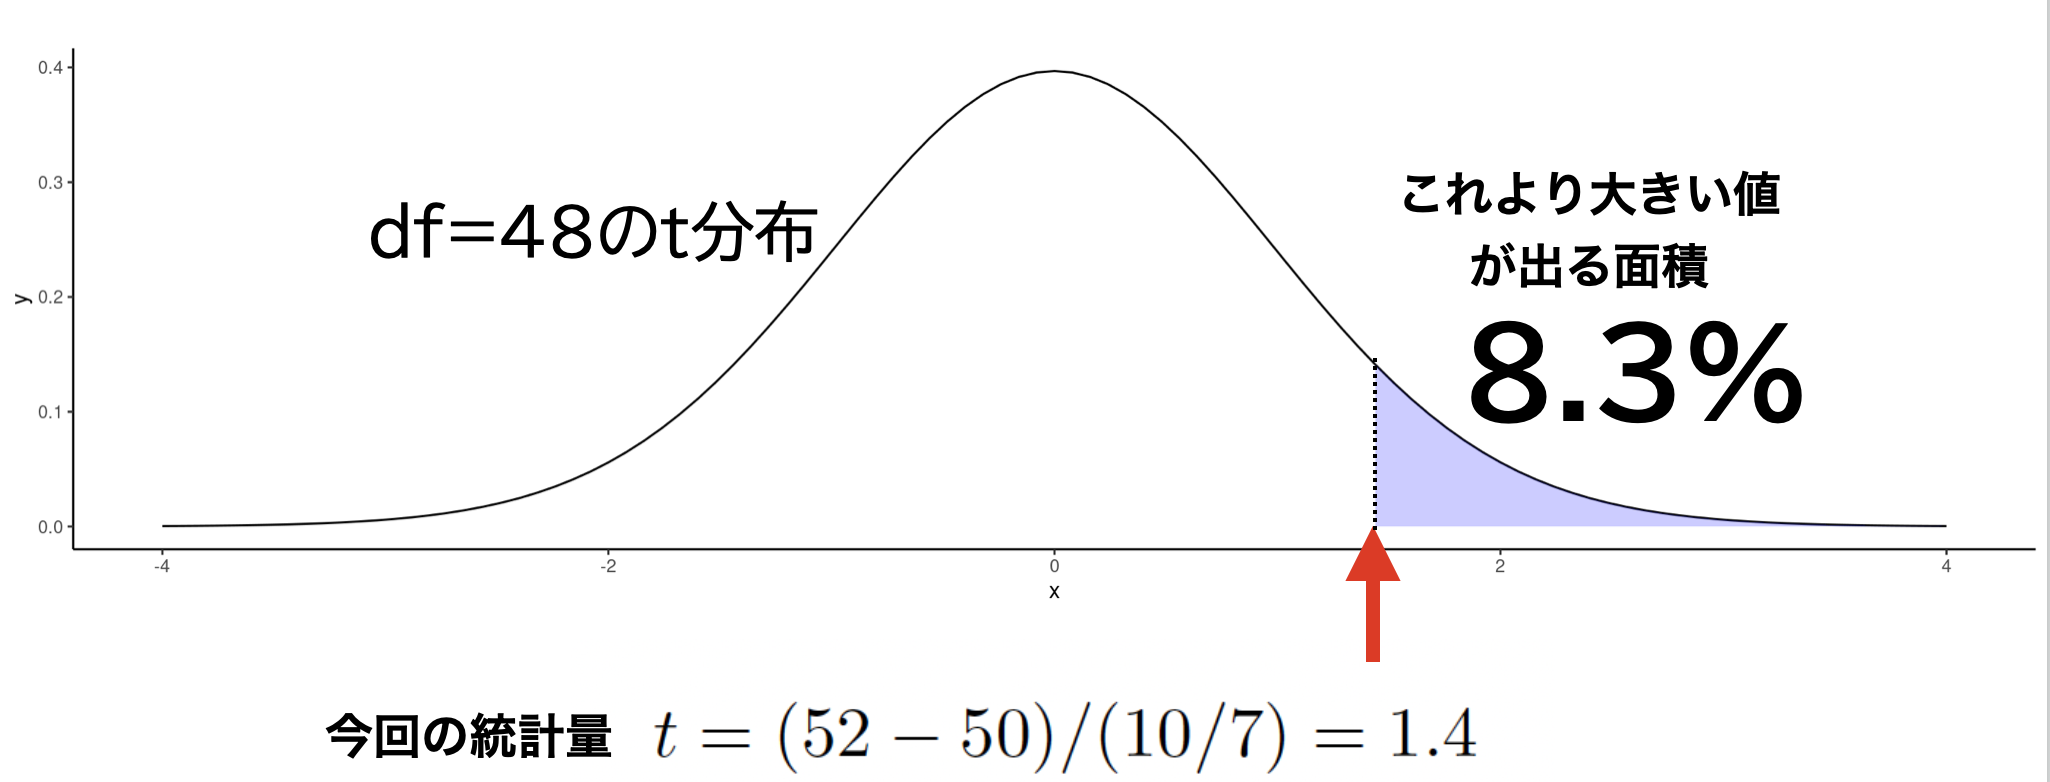
\includegraphics[keepaspectratio,width=0.8\linewidth]{../images/18_NHST/slide18_03.png}
	\caption{t分布をつかったときの棄却域と臨界値}
	\label{fig::18_02b}
\end{figure}



\subsection{When the mother SD is not understood}
The previous example was about the situation where the population standard deviation was known. I mentioned the same thing in Chapter \ref{m17_estimation_and_test}, but if the population parameters are known, it's not difficult to make estimates. The reason we make estimations is because we don't know the population parameters.

So, instead of using the population standard deviation, we will be using the sample standard deviation (the positive square root of the unbiased variance) as an estimate on behalf of the mother SD. In this case, since the (standard) normal distribution cannot be used, we will use the t-distribution based on the sample size. Let's try the same example with this approach. This time, we will need the sample standard deviation, which we will assume to be $\hat{\sigma}=10$.

The null hypothesis and alternative hypothesis are the same as earlier: either $\mu=50$ or $\mu \neq 50$. However, in this case, the test statistic used for inference is the t statistic.
Following convention for the criteria, let's set it to 5% for now.
The test statistic $t$ can be obtained by using the formula $t = \frac{\bar{X}-\mu}{\hat{\sigma}/\sqrt{n}}$, without altering the TeX code.
\[ t = (52-50)/(10/7) = 1.4 \]
The text in Japanese translates to:

"This follows a $t$-distribution with $n-1=48$ degrees of freedom. Therefore, to find the probability of getting a number at least 1.4 or greater in a $t$-distribution with 48 degrees of freedom, we obtain $p = 0.08397194$. \footnote{This is calculated in R with the following command: \texttt{1-pt(1.4,df=48)}}. So it is 8.3%."

This is the decision. Since a probability greater than the 5% decision line was obtained, this is not a rare event. It's not unheard of, so it's a common occurrence. In other words, we can't say it's a large number that deviates from the mean.
We have shown the image related to this particular test in Figure \ref{fig::18_02b}. We drew a t-distribution with 48 degrees of freedom and indicated the realized value of the test statistic. You can make a judgment on whether the realized value falls within the rejection region or not, or you can directly calculate the probability, as we did in this case, to determine if it is 5\% or not. It may seem easier to directly calculate the probability, but historically, when there were no machines available to do so, people used to look at tables of numbers to make judgments. In the column on number tables in Lecture \ref{m07_probability}, on page \pageref{NumberTable}, we introduced these tables and explained that they were used to determine if one fell within the rejection region based on the size of the critical values, which was a common practice at the time.
\begin{figure}[ht]
    \centering
    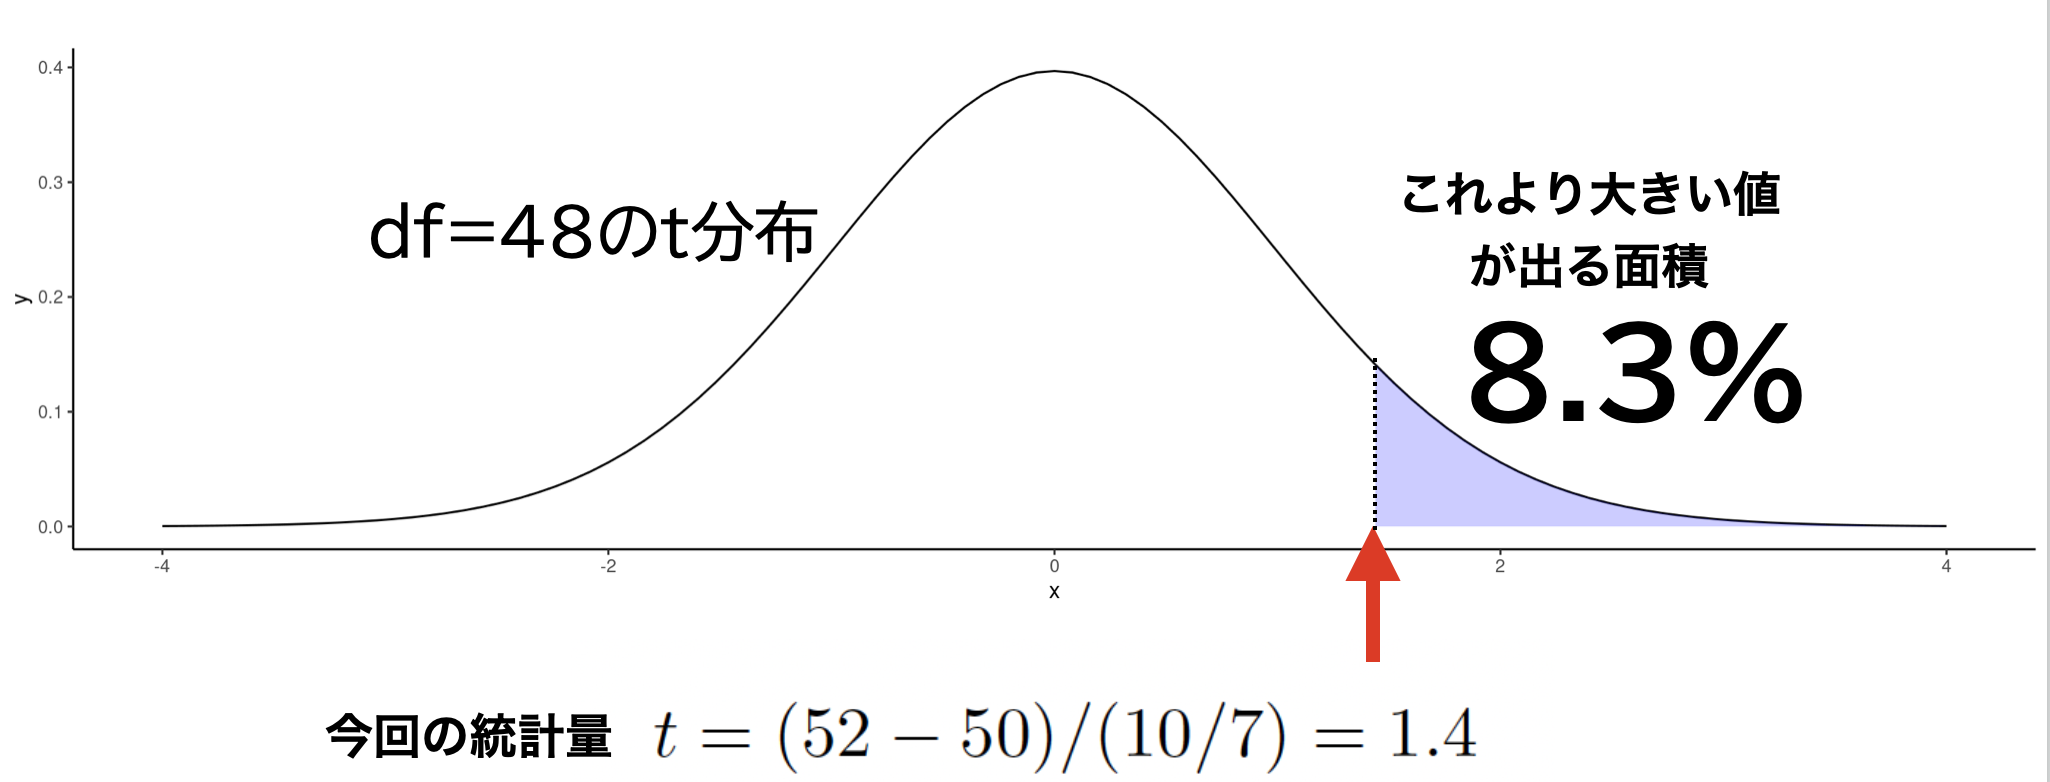
\includegraphics[keepaspectratio,width=0.8\linewidth]{../images/18_NHST/slide18_03.png}
    \caption{Rejection region and critical value when using t-distribution}
    \label{fig::18_02b}
\end{figure}



How was it? In this data, we were unable to reject the null hypothesis, whether or not we knew the population standard deviation. This may seem like a roundabout way of saying things or be difficult to grasp. Therefore, I'd like to consider another case, an example of correlation coefficients, and gradually become more accustomed to the procedures and ways of drawing conclusions.

\section{Testing Correlation Coefficients}
Let's now talk about the significance test of correlation coefficients.
In psychology, it is not uncommon to study not only the estimation of the mean value, but also the correlation coefficient. If it involves comparison before and after an intervention or between groups, such as in experiments, we talk about the mean value. However, in cases where the causal relationship is unclear and there may be some connection, exploratory research is often conducted to understand the phenomenon. For example, there may be a relationship between depression and wake-up time. Self-esteem may be related to academic performance. Attitudes towards love may be related to personality, etc. It seems like we are getting into psychology-like topics!

Let's consider the last example of studying the relationship between attitudes towards love and personality. Suppose there are measures to assess "positive attitudes towards love" and whether someone has an extroverted personality based on previous research\footnote{Although briefly mentioned here, developing and utilizing psychological measures to assess psychological states is an important area of research in psychology. This field is called \keytermE{psychological measurement}, and it involves examining responses to survey items using factor analysis models or structural equation modeling. Since these measures attempt to assess something invisible, it is crucial to evaluate whether they are measuring what they intend to measure. Additionally, there are many psychological measures that have been published and are publicly available, but when borrowing them for research, it is essential to have a critical attitude, such as questioning whether the measure is assessing what one wants to measure and whether it would produce the same results for one's research subjects.}. Using these measures, we recruited 20 participants and obtained their responses to calculate the sample correlation coefficient, resulting in a value of $r=0.5$ (referring back to the calculation of correlation coefficients from Lesson \ref{m08_CorrelationCausation}).\footnote{By the way, the expected value of the sample correlation coefficient (i.e., the average value of sample correlation coefficients obtained from repeated sampling) does \textbf{not} match the population correlation coefficient. Therefore, one must calculate the unbiased correlation coefficient similarly to how one would calculate unbiased variance, but because it cannot be expressed in a simple formula, it is customary to estimate it using the sample correlation coefficient alone \citep{Haebara200206,Hirakawa2021}. Moreover, when conducting interval estimation, one must consider the standard error of the sample correlation coefficient. The estimated standard error of the sample correlation coefficient, denoted $\hat{\sigma}_r$, is given by the following formula.}
"You are a translator."
In this case, $\hat{\sigma}_r = \frac{1-0.5^2}{\sqrt{20} }= 0.1677$. However, since the sample distribution of the sample correlation coefficient is not normal, Fisher's z transformation is necessary to perform interval estimation.

Well, the sample correlation coefficient is $r=0.5$, but what about the population correlation coefficient? Can we say that these two variables are also related in the population? To extend our discussion from the sample to the population, we need to make an estimation and conduct a hypothesis test to reach a conclusion. Let's move on with the steps of hypothesis testing.

Hypothesis setting: In the case of correlation coefficients.
The first step is to set the hypothesis. A null hypothesis and an alternative hypothesis are necessary. The null hypothesis is a hypothesis that is deemed to be Null, so in this case, it would be "there is no correlation".
The population correlation is represented by the Greek letter $\rho$ (pronounced "rho"), so mathematically, the null hypothesis is $H_0: \rho = 0$. This is a strong assertion that the population correlation is exactly equal to zero.
The alternative hypothesis to this is its negation, therefore $H_1:\rho \neq 0$. Since there is already a model comparison between these two, the null hypothesis is quite specific, but in terms of hypothesis testing, we have no choice but to approach it in this way.

The essence of the story is that null hypothesis testing uses the logic of proof by contradiction. First, assume the world of the null hypothesis, and then if something strange happens according to that assumption, reject the null hypothesis. Let's imagine a world where the population correlation is zero - fortunately, we can now easily simulate this using computers. Assume a world where the correlation coefficient is zero and take a sample of 20 people from there.

\begin{figure}[ht]
    \centering
    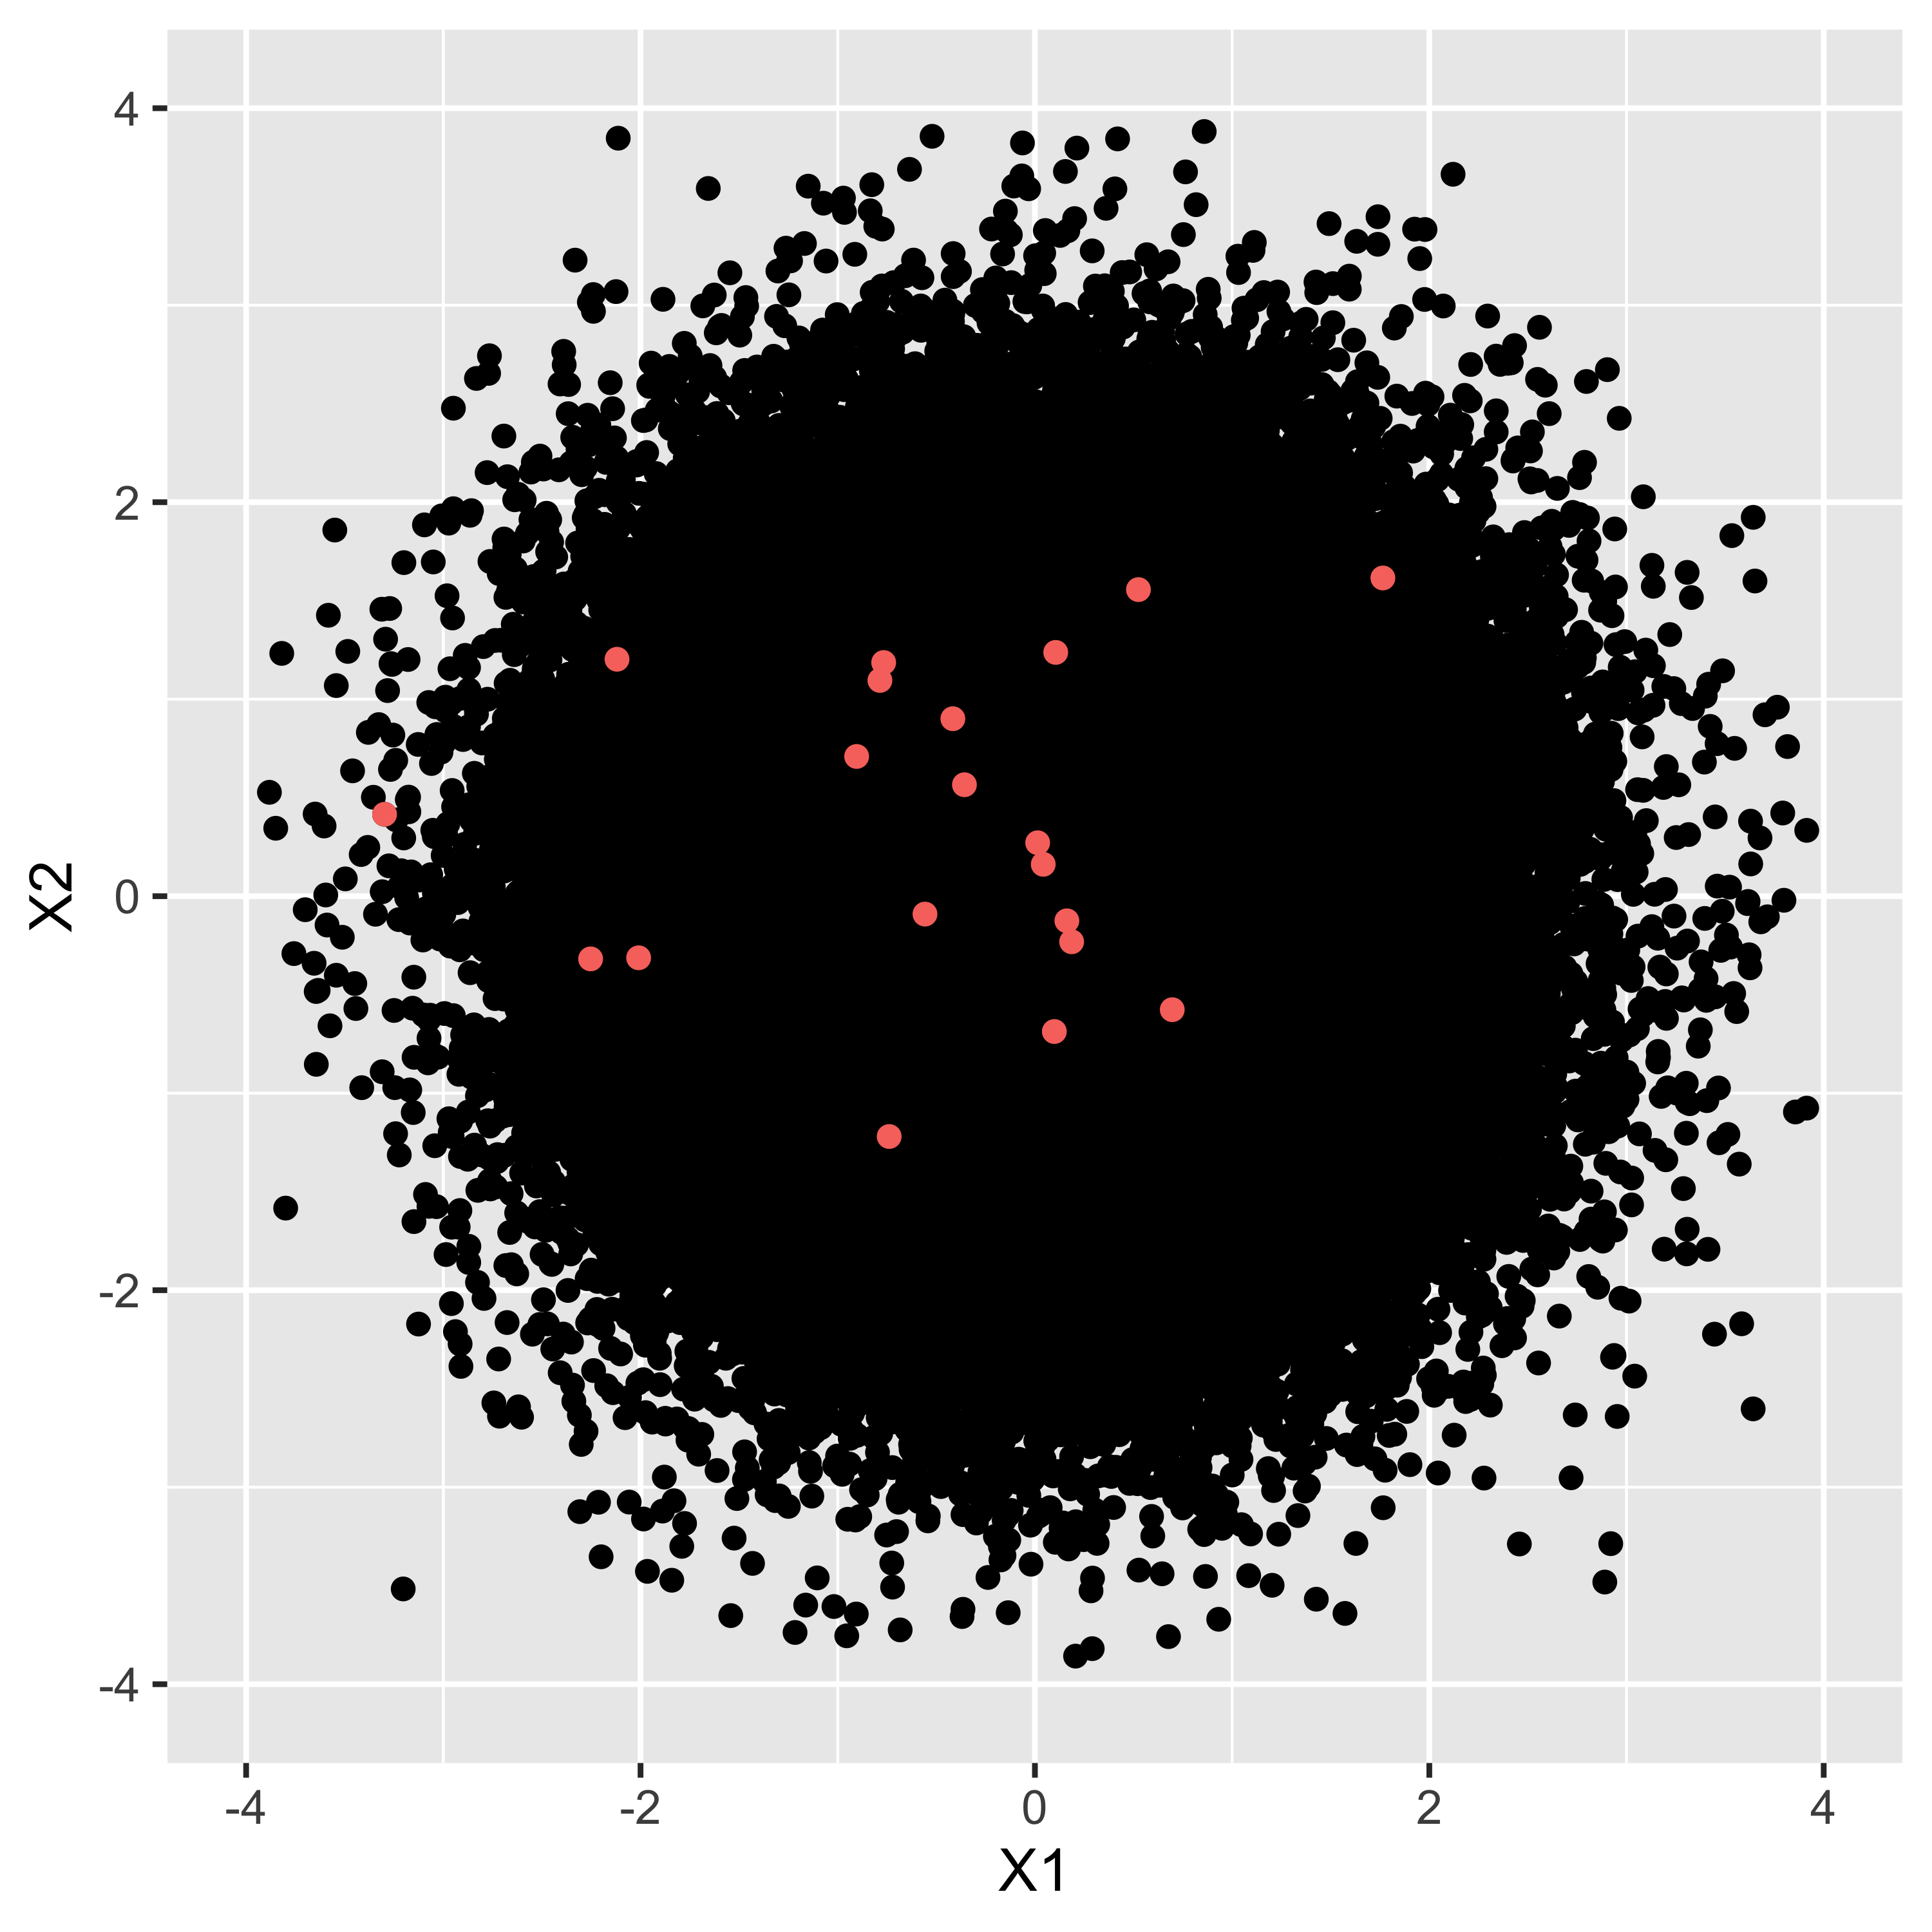
\includegraphics[keepaspectratio,width=0.8\linewidth]{../images/18_NHST/Rplot18_01.png}
    \caption{Example of taking a sample of size $n=20$ from a population with parent correlation $\rho=0$}
    \label{fig::18_01}
\end{figure}


What is shown in Figure \ref{fig::18_01} is an example of randomly selecting 20 points from 100,000 generated random numbers from a world with zero population correlation $\rho=0$. The cluster of black dots is almost circular, representing data with no correlation between the two variables. The small red dots represent the 20 randomly selected points, and the sample correlation coefficient for these 20 points was $r=0.143$. Although it would be ideal for $r$ to also be zero since it is a sample from a world with $\rho=0$, it is not always exactly zero when only certain samples are taken. When repeating this type of sample selection multiple times, the sample correlation coefficient will take various numbers such as $r_2=0.32, r_3=-0.46, r_4=-0.26$, etc. This distribution becomes the sample distribution.

In this way, assuming "the population correlation is $\rho = 0$", we consider what the sample distribution will be when a sample is taken, and then consider the probability that the sample correlation coefficient obtained this time (0.5 in this example) will occur. If the probability is very low, it means that something rare happened with the data in front of us, so we reject the null hypothesis that assumes "the population correlation is $\rho = 0$". This is where the proof by contradiction comes in. It should also be noted that it is difficult to assume the null hypothesis as "there is a population correlation!" because while there are countless levels of correlation that can be considered "existing", it is unique when the correlation "does not exist".

Establishing the test statistic

Here, it is known that the sample distribution of the sample correlation coefficient follows a t-distribution with degrees of freedom of $n-2$\footnote{Again, let's just borrow the result from mathematical statistics!}. However, instead of using the correlation coefficient as it is, it is necessary to transform the sample correlation coefficient using the following equation.

\[ t = \frac{r\sqrt{n-2}}{\sqrt{1-r^2}} \]

Setting Criteria for Judgment
As is customary, let's set it to 0.05 (5%).

Calculation of test statistics.

In this example,

\[ t = \frac{0.5 \times \sqrt{18}}{\sqrt{1-0.25}} = 2.44949 \]

You are a translator.

\paragraph{Now, for the judgement}

What is the probability of obtaining a number larger than $t=2.45$ from a t-distribution with 18 degrees of freedom? Using the calculation \footnote{In R, this is done by typing \texttt{1-pt(2.45,df=18)}.}, we get a probability of $p=0.01237173$. We are also considering the probability of obtaining a biased correlation coefficient greater than 0.5, given that $\rho=0.0$. Since we are only concerned with $|r|>0.5$, which is symmetrical, we should consider $p=0.0124 \times2=0.0248$. In any case, the probability of obtaining a sample correlation coefficient with an absolute value greater than 0.5 is a very small number compared to the 5% cutoff point, and we may confidently conclude that this is a rare event. Therefore, the null hypothesis is unlikely to be valid. In fact, it is highly unlikely to obtain a sample correlation coefficient of $r=0.5$ if the population correlation coefficient is $\rho=0$. We must therefore reject the null hypothesis and accept the alternative hypothesis. Figure \ref{fig::18_03b} illustrates the relationship between the t-distribution, the critical value, and the observed value, so please refer to it for confirmation.

\begin{enumerate}
    \item 標本平均から推測した母平均の95 \%信頼区間はどのような値になりますか。標本分布に照らし合わせて考えてください。
    \item 母集団に照らし合わせた時，今回の標本平均以上の数字が出てくる確率はどれぐらいですか。母集団分布に照らし合わせて考えてください。
    \item 有意水準を5\%として帰無仮説検定をします。この時の帰無仮説と対立仮説はそれぞれどのようになりますか。
    \item 有意水準を5\%として帰無仮説検定をします。結論として，どちらの仮説が採択されますか。
\end{enumerate}




How was it?
Although it uses a slightly different logic from interval estimation, by setting criteria for judgment and pitting two hypotheses (models) against each other, it is now possible to make a determination.
Next time, I would like to consider the reporting methods for this test result and the issues brought about by the null hypothesis testing.

\section{Task}
"Let's test the average value when the mother standard deviation is known."
The sample mean was 45 when a sample of size 16 was taken from a population with a mean of 40 and a standard deviation of 10.
I would like to determine whether the inferred mean from this sample is significantly different from that of the population.
At this time, please answer the following question.
\begin{enumerate}
    \item 標本平均から推測した母平均の95 \%信頼区間はどのような値になりますか。
    \item 母集団に照らし合わせた時，今回の標本平均以上の数字がこの母集団から得られる確率はどれぐらいでしょうか。
    \item 有意水準を5\%として帰無仮説検定をします。この時の帰無仮説と対立仮説はそれぞれどのようになりますか。
    \item 有意水準を5\%として帰無仮説検定をします。結論として，どちらの仮説が採択されますか。
\end{enumerate}


Using t-distribution for interval estimation
The population mean is 40, and although the population standard deviation is unknown, a sample of size $n=16$ was taken with a sample mean of $\bar{X}=45$ and an unbiased sample standard deviation of $\hat{\sigma}=9$.
I would like to determine whether the inferred mean from this sample is significantly different from the population.
Please answer the following question at this time.
\begin{enumerate}
    \item What is the 95\% confidence interval for the population mean inferred from the sample mean?
    \item What is the probability of obtaining a number greater than the sample mean from this population when compared to the entire population?
    \item Conduct a null hypothesis test with a significance level of 5\%. What are the null and alternative hypotheses in this case?
    \item Conduct a null hypothesis test with a significance level of 5\%. In conclusion, which hypothesis is accepted?
\end{enumerate}


Using t-distribution for testing correlation coefficients.
Suppose we have a sample size of $N=49$ and obtained a sample correlation coefficient of $r=0.3$. We want to determine whether this sample correlation coefficient is statistically significant or not.
At this time, please answer the following question.
\begin{enumerate}
	\item What are the null hypothesis and alternative hypothesis when conducting a significance test with a significance level of 5%?
	\item When conducting a significance test with a significance level of 5%, which hypothesis is accepted as a conclusion?
\end{enumerate}


\end{document}
